%! Author = a
%! Date = 1/27/25

% Preamble
\documentclass[11pt,a4paper]{report}

% Packages
\usepackage{amsmath}
\usepackage{hyperref}
\usepackage[most]{tcolorbox}
\usepackage{graphicx}
\usepackage{float}
\usepackage{subcaption}
\usepackage{textcomp}
\usepackage{siunitx}
\usepackage{tikz}
\usepackage{mathtools}
\usepackage{multicol}
\usepackage{xifthen} % For conditional statements


\newtcolorbox{joke}[1][]{colback=blue!10!white,
    colframe=blue!80!black,fonttitle=\bfseries,
    colbacktitle=blue!85!black,enhanced,
    attach boxed title to top center={yshift=-2mm},
    title={Giggle Corner}
}

\newtcolorbox{note}[1][]{colback=yellow!10,
    colframe=yellow!80!black,
    fonttitle=\bfseries,enhanced,
    title={Note}
}

\usetikzlibrary{shapes.geometric, arrows, positioning}
\tikzset{every node/.style={node distance=2em}}

\tikzstyle{terminator} = [
rectangle,
draw,
text centered,
rounded corners,
%	minimum width=5em,
minimum height=2.5em,
text width=6em,
]

\tikzstyle{process} = [
rectangle,
draw,
text centered,
minimum height=3em,
text width=6em,
]

\tikzstyle{decision} = [
diamond,
draw,
text centered,
aspect=2,
minimum height=3em,
minimum width=12em,
text width=6em,
]

\tikzstyle{data} = [
trapezium,
draw,
text centered,
trapezium left angle=60,
trapezium right angle=120,
minimum height=3em,
text width=4em,
]
\tikzstyle{arrow} = [thick,--]

% Document
\begin{document}
	\title{Hitchhiker's Guide to China}
	\author{Brayko Timofey \\ Miasoedov Artemii}

	\maketitle
	\tableofcontents

	\part[Russia]{Russia}\label{part:ru}
	%! Author = a
%! Date = 1/27/25




\chapter{BIT Application}\label{ch:ru_application}

After you were qualified for the exchange program,
you need to sign up for an exchange program on
\href{https://apply.isc.bit.edu.cn/apply/}{the BIT website}.
Go to the website,
register and click on \textit{Start Application}.

\begin{note}
    Google is banned in China.
    We recommend to use Yandex or University email
    for registration and other purposes.
\end{note}







\section{Study Plan}\label{sec:study_plan}

Firstly, choose \textcircled{1} \textbf{``Exchange and Visiting Programs``},
as you apply for the exchange program.
On the next page if you are a bachelor student (undergraduate),
choose \textcircled{2} \textbf{``General Visiting Student``}.
For masters, choose \textbf{``Senior Visiting Student``}
Fig~\ref{fig:ru_student_type}.


\begin{figure}[htbp]
    \centering
    \begin{subfigure}[c]{0.49\textwidth}
        \centering
        
\includegraphics[width=\textwidth]{01_russia/imgs/app_1}
    \end{subfigure}
    \hfill
    \begin{subfigure}[c]{0.49\textwidth}
        \centering
        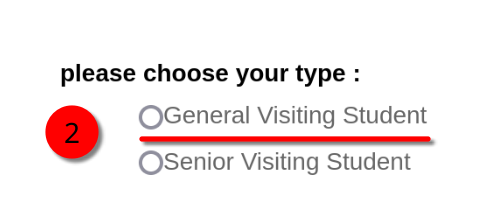
\includegraphics[width=\textwidth]{01_russia/imgs/app_2}
    \end{subfigure}
    \caption{Study Program}
    \label{fig:ru_student_type}
\end{figure}


After, you should specify the Department and Major.
For Department \textcircled{1} and Major \textcircled{2} choose
\textbf{``Computer Science and Technology``}.
Don't forget to specify the English language \textcircled{3}!
Start the search \textcircled{4} and choose appropriate study plan \textcircled{5}.
Additionally, pay attention to application period!
Maybe the application period not started yet.
Fig~\ref{fig:ru_study_plan}


\begin{figure}[htpb]
    \centering
    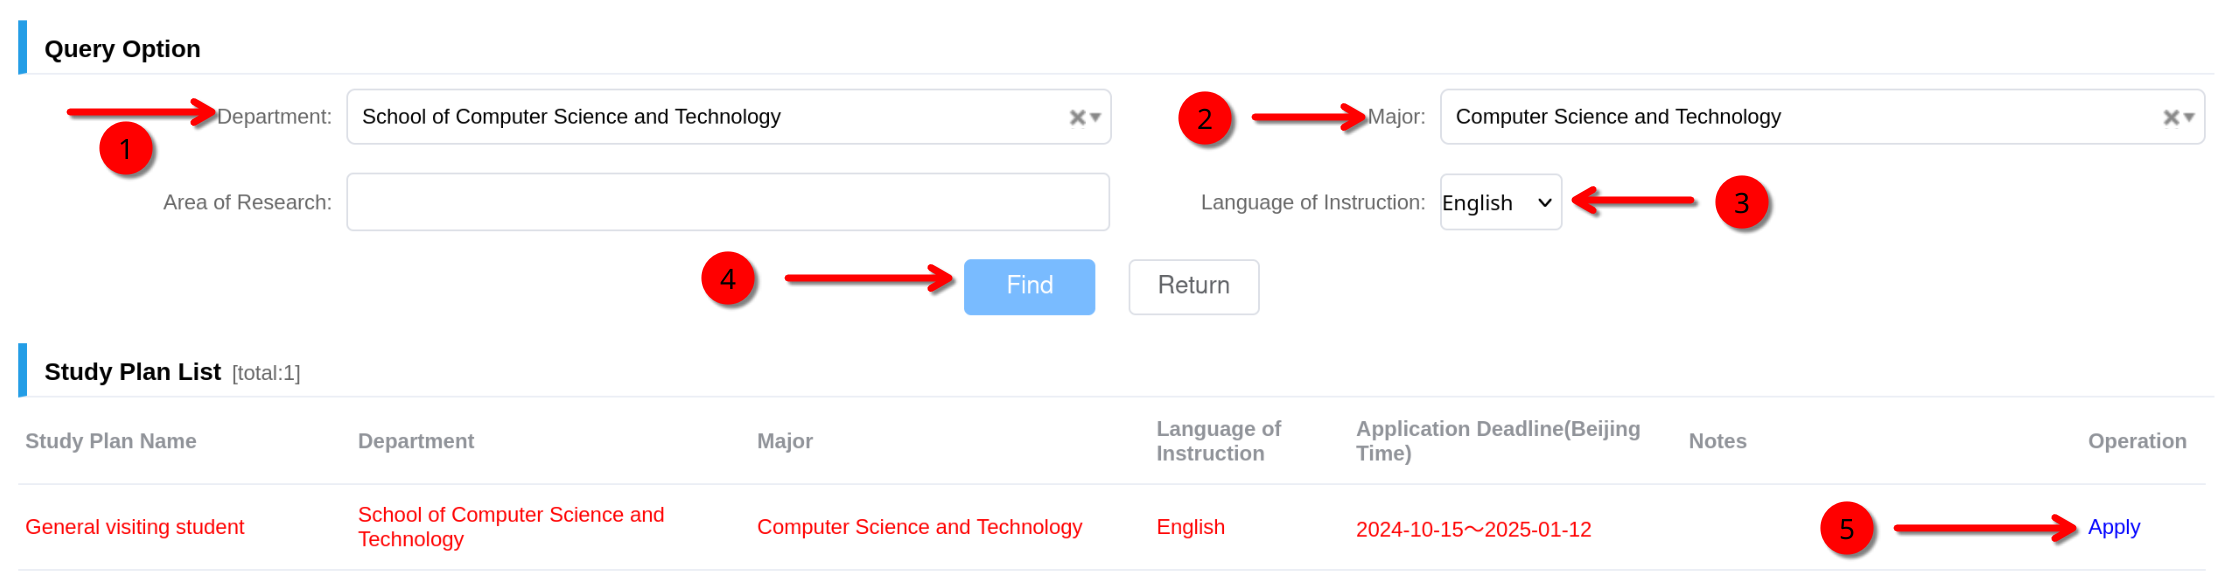
\includegraphics[width=\textwidth]{01_russia/imgs/app_3_study_plan}
    \caption{\centering Study Plans}
    \label{fig:ru_study_plan}
\end{figure}








\section{Personal Information}\label{sec:ru_personal_info}

This section not that hard, but some points should be clarified!
Fig~\ref{fig:ru_pers_info}

\begin{enumerate}
    \item Fill the name and surname according to international passport.
        If you still don't have it, you can check spelling
        \href{https://www.gosuslugi.ru/help/faq/foreign_passport/100359}{HERE}.

    \item \textbf{Highest Level of Education}: Bachelor

    \item \textbf{Final Education Institution}: Innopolis University

    \item \textbf{Occupation}: Student

    \item \textbf{Chinese Name}.
        If you don't have Chinese name yet, leave field blank.
        The Chinese coordinator will give you Chinese names that match the real ones. \\
        \textbf{For example}: Timofei - MoFei, Artur - AnTeng (it may sound not that similar)

    \item \textbf{Employer or Institution Affiliated}: Innopolis University
\end{enumerate}


\begin{figure}[H]
    \centering
    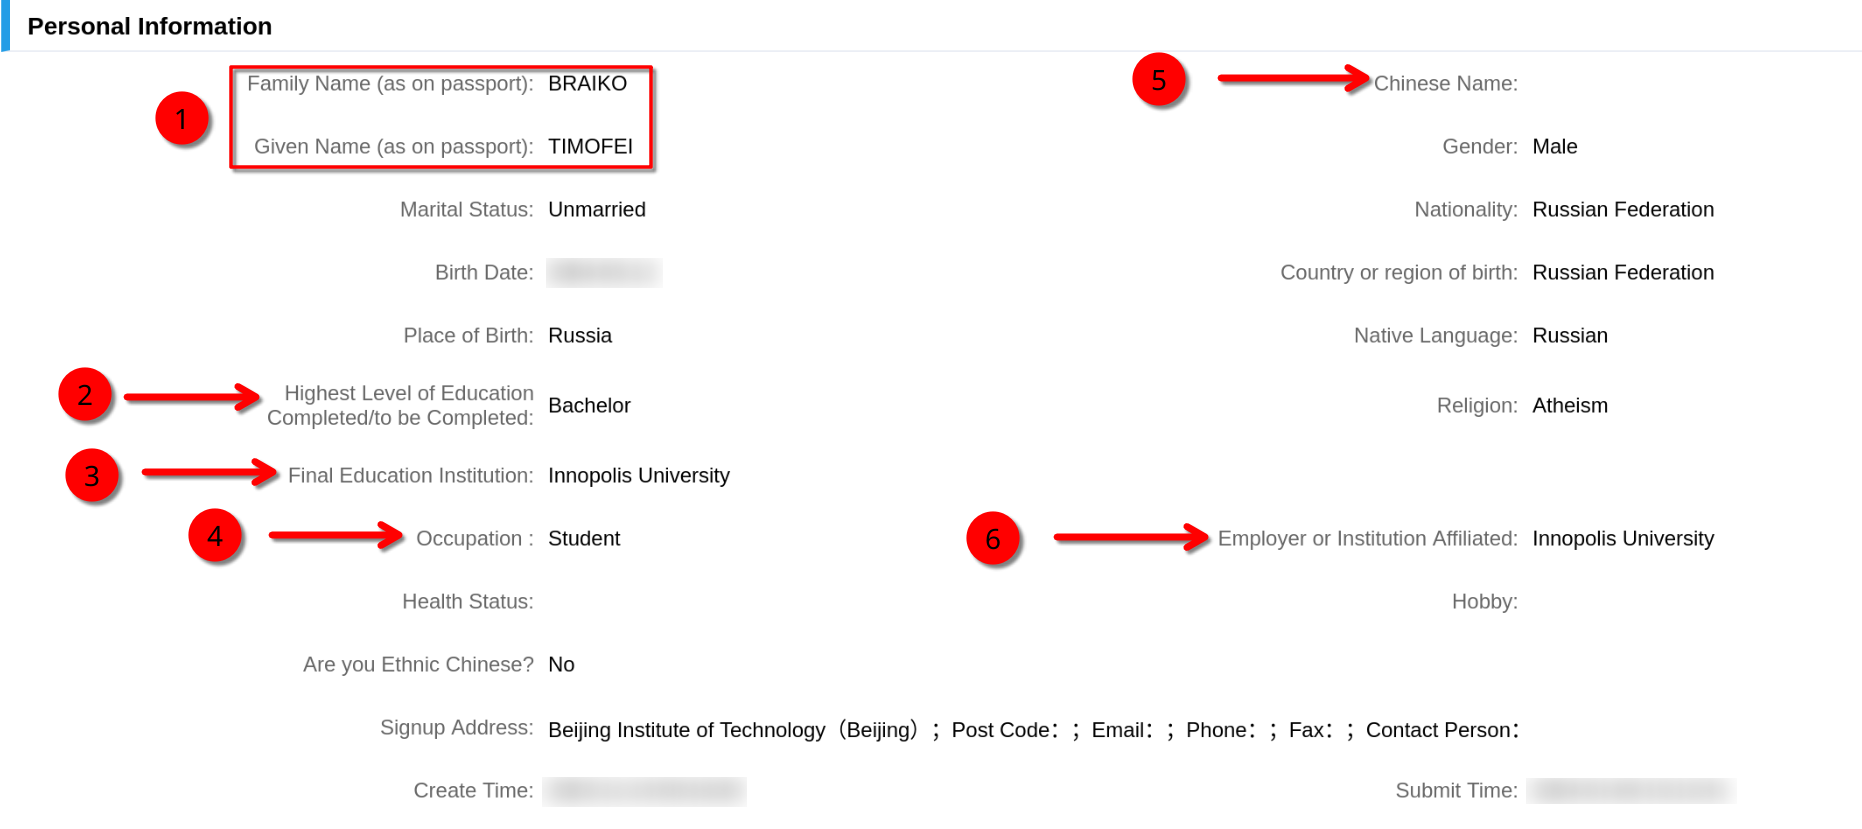
\includegraphics[width=\textwidth]{01_russia/imgs/app_4_personal_info}
    \caption{\centering Personal Information}
    \label{fig:ru_pers_info}
\end{figure}









\section{Passport}\label{sec:ru_passport}

In this section, you fill in your international passport details.
You should get and submit your international passport before application deadline.
Otherwise, write to Innopolis coordinator.
As of 2024, it's Veronika Mezenova (@Nika\_Mezenova)

Regarding field \textbf{Location of Visa Office}.
At the end of 2024, a Chinese visa can be obtained in the following places:

\begin{itemize}
    \item \textbf{Embassy in Russia Federation} - Moscow
    \item \textbf{Consulate in St.Petersburg}
    \item \textbf{Consulate in Yekaterinburg}
    \item \textbf{Consulate in Khabarovsk}
    \item \textbf{Consulate in Vladivostok}
\end{itemize}


\begin{note}
    At the time of writing, a visa cannot be obtained in Kazan.
\end{note}









\section{Language Proficiency}
Enter the exam results.
Please note that if you have passed the IELTS or TOEFL yourself,
they are valid for only two years.
If you passed inner-university exam choose IELTS, as it's based on IELTS exam.
Issue date is printed on certificate Fig~\ref{fig:ru_lang_prof}.


\begin{figure}[H]
    \centering
    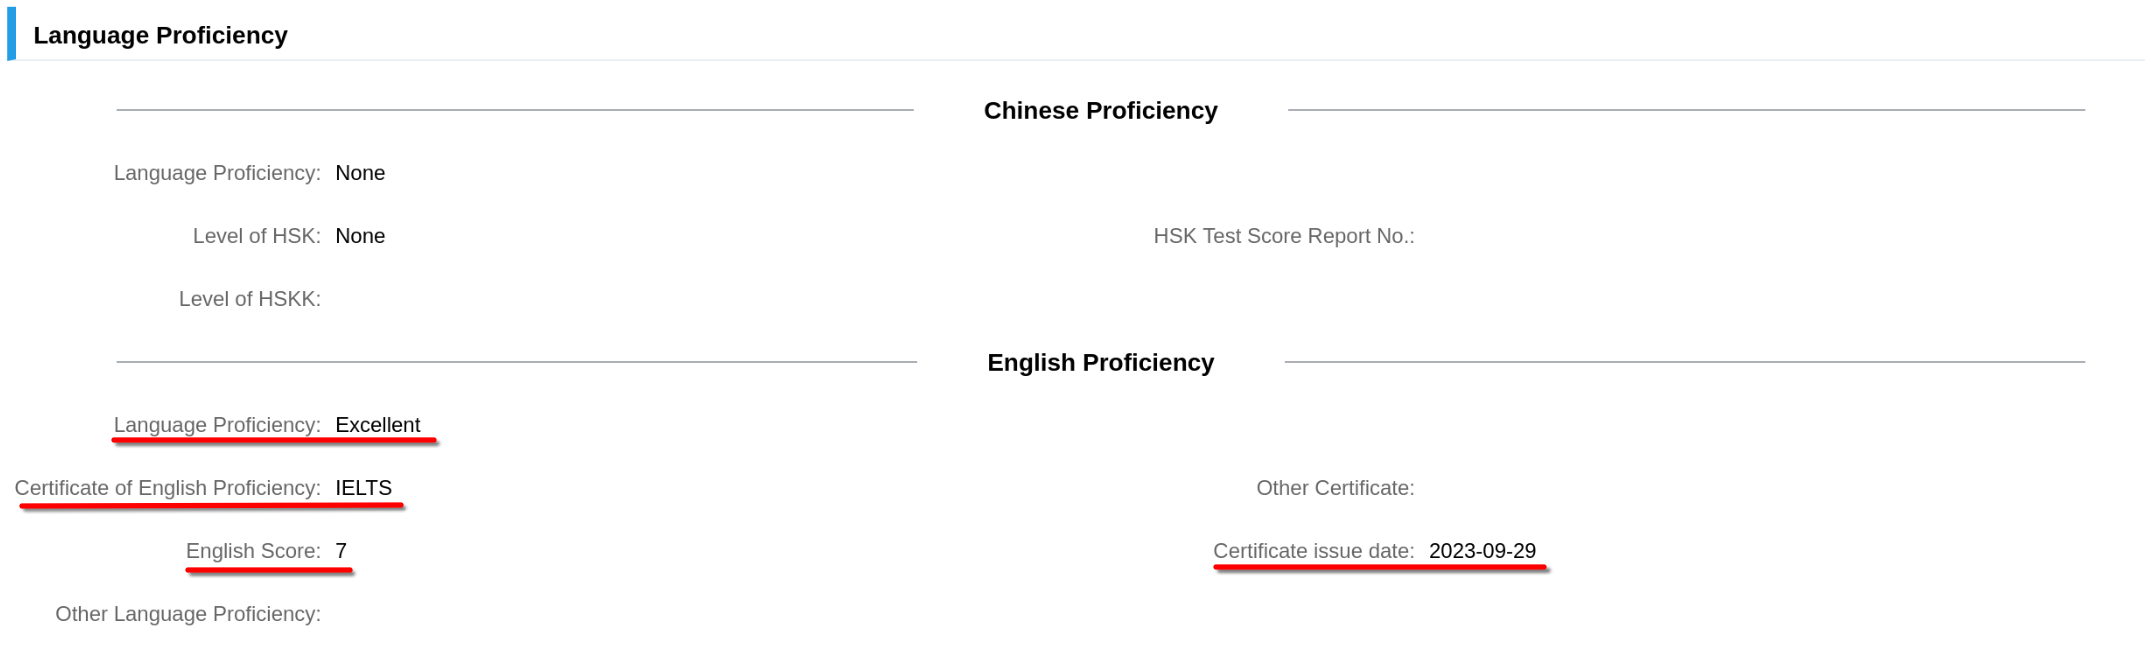
\includegraphics[width=\textwidth]{01_russia/imgs/app_5_language}
    \caption{\centering Language Proficiency}
    \label{fig:ru_lang_prof}
\end{figure}









\section{Recommender}
Specify the head of the department here.
For this moment, he is Petr Zhdanov Fig~\ref{fig:ru_recommender}.

\begin{itemize}
    \item \textbf{Source:} Others - Head of the International Relation Office
    \item \textbf{Name:} Petr Zhdanov
    \item \textbf{Organization:} Autonomous noncommercial organization of higher education ``Innopolis University``.
    \item \textbf{Phone Number:} +7 843 203 92 53
    \item \textbf{Relationship with applicant:} Head of the International Relation Office
    \item \textbf{Email:} pe.zhdanov@innopolis.ru
\end{itemize}


\begin{figure}[H]
    \centering
    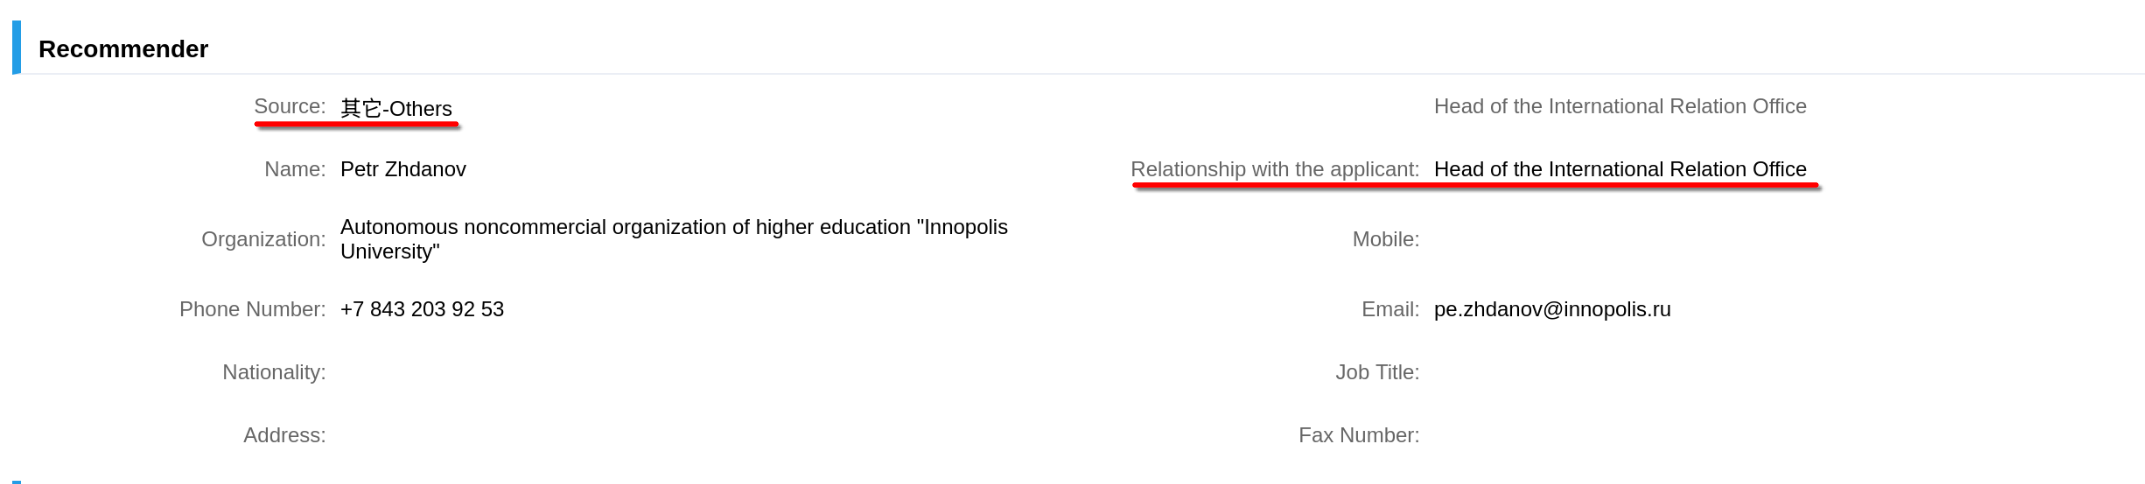
\includegraphics[width=\textwidth]{01_russia/imgs/app_6_recommender}
    \caption{\centering Recommender}
    \label{fig:ru_recommender}
\end{figure}







\section{Educational Background}\label{sec:ru_edu}

This section not so important, if you're bachelor.
Just specify your school.
Below you can see example in Fig~\ref{fig:ru_edu_back}.
Probably not that many details are needed.


\begin{figure}[H]
    \centering
    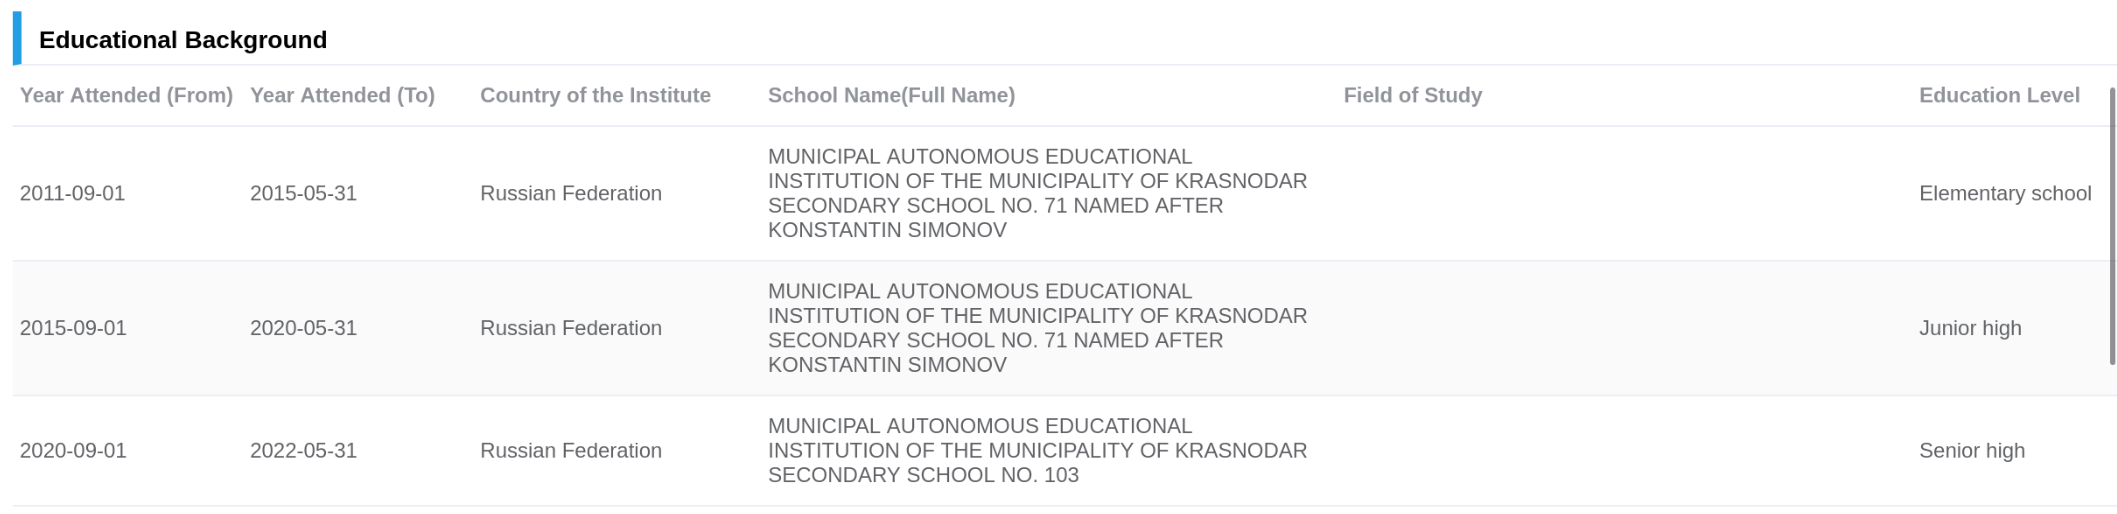
\includegraphics[width=\textwidth]{01_russia/imgs/app_edu_back}
    \caption{\centering Educational Background}
    \label{fig:ru_edu_back}
\end{figure}







\section{Family}\label{sec:ru_family}
Here, specify two relatives (parents)
with their contacts and place of work.


\begin{joke}
The Chinese Party prohibits specifying more than two relatives,
because one family means one child.
Otherwise, the Chinese Party will take away the
cat-wife and a bowl of rice.
\end{joke}





\section{Financial Supporter and Guarantor}\label{sec:ru_fin_supp}
Financial Supporter and Guarantor should be the same person.
This is someone who will financially support you (does not have to live in China).
Basically it's one of the parents.





\section{Addresses}\label{sec:ru_addr}

\begin{itemize}
    \item \textbf{Permanent Address} - address in internal passport
    \item \textbf{Current Postal Address} - Place of current residence.\\
        Innopolis Dorms or Kazan if you live there.
    \item Zip Code for Innopolis: 420500
\end{itemize}







\section{How to collect Admission Notice}\label{sec:ru_adm_not_delivery}

It's the most crucial document you need for exchange program.
Admission notice is enrolment document required to get \textit{Study Visa},
go through border control in China, apply for a bank card and so on.

If you have two options as shown in Fig~\ref{fig:ru_collect_adm_not},
\textbf{it's better to choose deliver option}.
In the end, Admission Notice will be sent by email.
Highly likely this question doesn't affect on anything.
However, better choose delivery option, to not screw up.


\begin{figure}[H]
    \centering
    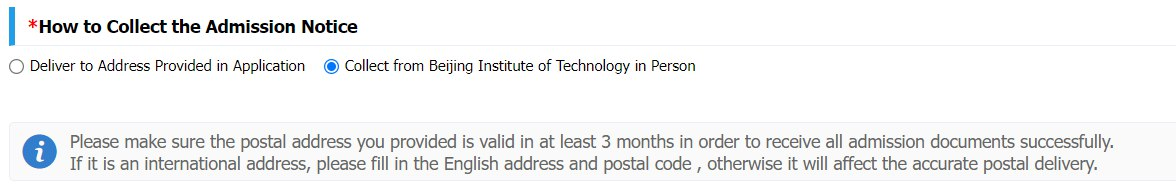
\includegraphics[width=\textwidth]{01_russia/imgs/app_adm_notice}
    \caption{\centering Options to collect Admission Notice}
    \label{fig:ru_collect_adm_not}
\end{figure}






\section{Uploading Documents}\label{sec:ru_upload_docs}

\begin{itemize}
    \item \textbf{Passport} - PDF with main and visa pages

    \item \textbf{Transcripts} - You should have it by this time.
        Otherwise, get it via
    \href{https://my.university.innopolis.ru/profile/edu-certs/create}{Innopolis website}.

    \item \textbf{Proof of Language Proficiency} - Results of English exam.

    \item \textbf{Recommendation Letter} - The same document if you pass inner-exam.
    If you're master student, get it from your supervisor.

    \item \textbf{Physical Examination Records} - See chapter~\ref{...}.

    \item \textbf{Non-Criminal Record} - Chinese guys will do it for you.
\end{itemize}
	%! Author = t
%! Date = 2025-02-05

\chapter{Physical Examination}\label{ch:ru_medical_examination}

\section{Intro}\label{sec:ru_}


The Chinese don't want you to come sick
(otherwise they'll have Vietnamese flashbacks),
so you need to collect some tests.
If you


\begin{note}
    Start preparing it immediately after
    you were nominated on exchange program by Innopolis.
    It takes a lot of time and efforts.
\end{note}



\section{Medical tests}\label{sec:ru_medical_tests}

To fill out this examination properly,
you must take the following tests:
\begin{itemize}
    \item Photofluorography
    \item Electrocardiography (ECG)
    \item Rh blood group system
    \item Human Immunodeficiency Viruses (HIV)
    \item Syphilis
    \item A certificate from a psychiatrist and addictionologist (narcologist)
    \item \textbf{Additionaly:} Vaccination list
\end{itemize}


Unfortunately, doctors in Innopolis hospital cannot fill out this form.
To fill out the form you should go to hospital in Kazan:

\textbf{Address:} Chuikova 54, terminal 2, 1st entrance,
2nd floor, office 2.8. Opening hours are 8:00-16:00.
\href{https://yandex.ru/maps/-/CHeHe8KC}{Yandex Maps}











\section{Can't finish examination on time}

On BIT website, you have to submit a completed examination before a deadline.
If you cannot complete it before,
you should receive mail in inbox on BIT website and fill the document Fig~\ref{fig:ru_med_state}.


\begin{figure}[htpb]
    \centering
    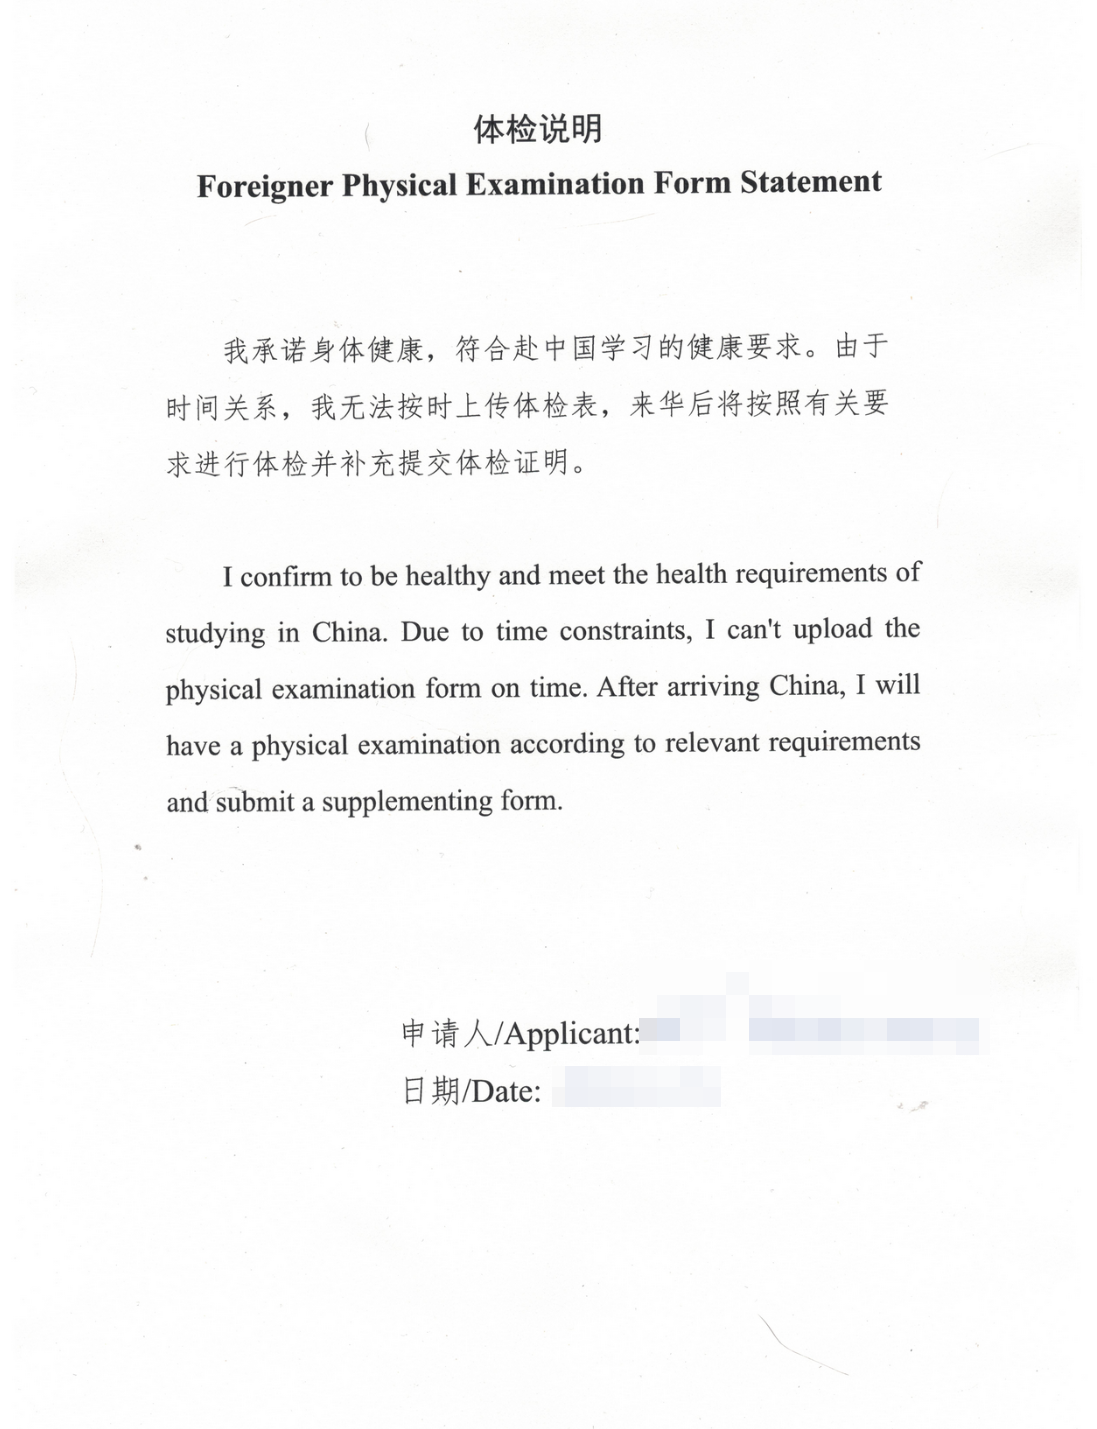
\includegraphics[width=0.8\textwidth]{01_russia/imgs/medical_statement}
    \caption{\centering Medical Examination Statement}
    \label{fig:ru_med_state}
\end{figure}

	%! Author = t
%! Date = 2025-02-20


\chapter{Visa}\label{ru:ru_visa}

All relevant information you can find on the website!
All guides and information highly-likely is up-to-date!
\begin{center}
\href{https://bio.visaforchina.cn/MOW3_RU/qianzhengyewu}{\Large Chinese Visa Application Service Center}
\end{center}


    %! Author = t
%! Date = 2025-02-20



\newcommand{\applinks}[2][]{
    \ifthenelse{\equal{#1}{}}
        {\href{#2}{PlatMarket}}
        {\href{#2}{PlatMarket}, \href{#1}{AppStore}}% If second parameter exists, return both
}

\chapter{Mobile Apps}\label{ch:ru_apps}

It's highly recommended to install several apps on your phone in advance!
List of all recommendations with links you can find in the end of this section.


\section{VPN}\label{subsec:ru_vpn}
China is famous for its \href{https://en.wikipedia.org/wiki/Great_Firewall}{Firewall},
so you better be ready to use VPN daily!
Here's a short list of banned websites and apps:

\begin{multicols}{2}
\begin{itemize}
    \item Telegram
    \item What's App
    \item Wikipedia
    \item Google
    \item YouTube
    \item Reddit
    \item StackOverflow
    \item GitHub (not banned, but really slow)
    \item HuggingFace
\end{itemize}
\end{multicols}

\begin{enumerate}
    \item \textbf{Install N different VPNs on your phone.}
        One day your VPN might work well, but the other it won't connect at all.
        And the opposite situation might be for other VPN app.

    \item \textbf{Install Tor/TorBrowser} on your phone and laptop.
        It maybe not the fastest solution, but at least most stable option among free solutions.
        Telegram Bot for Bridges: \href{https://t.me/GetBridgesBot}{@GetBridgesBot}

    \item \textbf{Personal Server}.
        You can also configure your proxy server.
        Using the VLESS protocol is highly recommended, as other options might be banned immediately by Chinese Firewall.
\end{enumerate}




\section[Chinese Apps]{Chinese Apps}\label{sec:chinese-apps}
If you use IPhone, you can skip this Section!

Most of the following applications are Chinese,
and not all can be downloaded from the Play Market.
Therefore, you will often have to download applications from the Internet.

An alternative to this is to download the Chinese Tencent AppStore (Install it by yourown).
Of course, Chinese apps are nightmare, but it's still a solution
if you don't want to suffer with installation via the Internet.




\section[Messanger and Payments]{Messanger and Payments}\label{sec:messanger-and-payments}

\begin{itemize}
    \item \textbf{WeChat}.
    Allows message, buy tickets, order food, read news and so on.
    However, to register, a Chinese person must verify your account using a QR code.
    But still download the app in advance and try to register,
    maybe you'll be lucky enough to enter without a QR code.
    Otherwise, just postpone it until you arrive in China.

    \item \textbf{AliPay}.
    The most affordable option for paying application fee.
    In China, it mostly used among foreigners for payment, but accepted everywhere.
    First time you can use it for chatting too!
\end{itemize}




\section[Maps]{Maps}\label{sec:ru_maps}

Google is banned and Yandex Maps almost useless, but you need somehow navigate in China.


\begin{itemize}
    \item \textbf{Chinese Apps} like AMap.
        However, it supports only Chinese language.

    \item \textbf{OpenSource solutions} like \href{https://maps.me/}{Maps.Me} or \href{https://osmand.net/}{OsmAnd}.
        Help you to navigate around, but won't tell what's in mall.

    \item \textbf{MetroMan}.
        It's the most convenient app for Chinese metro.
        Again mostly developed for foreigners, but works perfect!
\end{itemize}




\section[Language]{Language}\label{sec:language}
Translator one of the most crucial tool (unless you know Chinese).
But Google is banned!
We recommend to use Yandex Translator and install Chinese Language in advance!
Also, we recommend to install vocabulary Pleco.

If you're willing to learn some basics of Chinese,
try to use HelloChinese.
It's similar to Duolingo, but helps learn Chinese better.



\section[AppList]{App List}\label{sec:ru_app_list}

\begin{itemize}
    \item WeChat -- \applinks[https://play.google.com/store/apps/details?id=com.tencent.mm]{https://apps.apple.com/us/app/wechat/id414478124}
    \item AliPay -- \applinks[https://play.google.com/store/apps/details?id=com.eg.android.AlipayGphone]{https://apps.apple.com/us/app/alipay-simplify-your-life/id333206289}
    \item Orbot -- \applinks{https://play.google.com/store/apps/details?id=org.torproject.android}
    \item AMap -- \applinks[https://play.google.com/store/apps/details?id=com.autonavi.minimap]{https://apps.apple.com/us/app/amap-global/id461703208}
    \item Maps.Me -- \applinks[https://play.google.com/store/apps/details?id=com.mapswithme.maps.pro]{https://apps.apple.com/us/app/maps-me-offline-maps-gps-nav/id510623322}
    \item MetroMan -- \applinks[https://play.google.com/store/apps/details?id=com.xinlukou.metroman]{https://apps.apple.com/us/app/metroman-china/id466351433}
    \item Pleco -- \applinks[https://play.google.com/store/apps/details?id=com.pleco.chinesesystem]{https://apps.apple.com/us/app/pleco-chinese-dictionary/id341922306}
    \item Hello Chinese -- \applinks[https://play.google.com/store/apps/details?id=com.hellochinese]{https://apps.apple.com/us/app/hellochinese-learn-chinese/id1001507516}
    \item TaoBao -- \applinks[https://play.google.com/store/apps/details?id=com.taobao.taobao]{https://apps.apple.com/us/app/taobao/id387682726}
\end{itemize}



	\part[China]{China}\label{part:cn}
	%! Author = a
%! Date = 1/27/25


\chapter{Arrival}\label{ch:cn_arrival}
\section[Roaming]{Roaming}\label{sec:cn_arrival_roaming}
Welcome to China!
If Airplane mode is disabled on your phone, you will receive SMS from your carrier with prices for their services.
Use of your home country carrier abroad may be costly, up to $\SI{1}{\textdollar\per\mega\byte}$ of the Internet traffic.
So, I would highly recommend you to disable the roaming option in the phone settings.

\begin{figure}[H]
	\centering
	\begin{tikzpicture}
%		\begin{scope}[on grid]
			\node (rich) [decision, below=of start] {Are you millionaire?};
			\node (roaming) [process, below left=of rich] {Disable roaming};
			\node (datasaver) [process, below right=of rich] {Enable data saver};
			\node (contact) [decision, below right=of roaming] {Alive? Want tell someone?};
			\node (sms) [process, below right=of contact] {Send SMS};
			\node (end) [terminator, below=of contact] {End}
%		\end{scope}

		\draw [arrow] (rich) -- node [anchor=south east] {no} (roaming);
		\draw [arrow] (rich) -- node [anchor=south west] {yes} (datasaver);
		\draw [arrow] (roaming) -- (contact);
		\draw [arrow] (datasaver) -- (contact);
		\draw [arrow] (contact) -- node [anchor=south west] {yes} (sms);
		\draw [arrow] (contact) -- node [anchor=east] {no} (end);
		\draw [arrow] (sms) -- (end);
	\end{tikzpicture}
	\label{fig:cn_arrival_roaming}
\end{figure}

You will still be able to send or receive SMS even with roaming disabled.

\end{document}
